\documentclass[10pt]{standalone}
%\usepackage[utf8]{inputenc}
\usepackage{pgfplots}
\pgfplotsset{compat=1.15}
\usepackage{mathrsfs}
\usetikzlibrary{arrows}
\pagestyle{empty}
\begin{document}
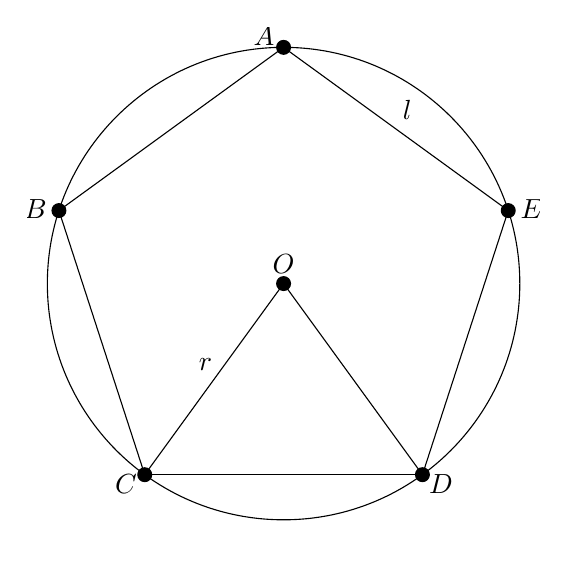
\begin{tikzpicture}[line cap=round,line join=round,>=triangle 45,x=0.5cm,y=0.5cm]

\clip(1.5,-0.5) rectangle (14.5,12.5);
\draw  (8.,6.) circle (3.cm);
\draw  (8.,12.)-- (2.293660902229079,7.8541019662496865);
\draw  (2.293660902229079,7.8541019662496865)-- (4.473288486245159,1.1458980337503175);
\draw  (4.473288486245159,1.1458980337503175)-- (11.526711513754835,1.1458980337503135);
\draw  (13.706339097770922,7.8541019662496865)-- (11.526711513754835,1.1458980337503135);
\draw  (13.706339097770922,7.8541019662496865)-- (8.,12.);
\draw  (8.,6.)-- (4.473288486245159,1.1458980337503175);
\draw  (8.,6.)-- (11.526711513754835,1.1458980337503135);

\draw [fill=black] (8.,6.) circle (2.5pt);
\draw[color=black] (8.0,6.5) node {$O$};
\draw [fill=black] (8.,12.) circle (2.5pt);
\draw[color=black] (7.5,12.3) node {$A$};
\draw [fill=black] (13.706339097770922,7.8541019662496865) circle (2.5pt);
\draw[color=black] (14.3,7.9) node {$E$};
\draw [fill=black] (4.473288486245159,1.1458980337503175) circle (2.5pt);
\draw[color=black] (4.0,0.9) node {$C$};
\draw [fill=black] (2.2936609022290795,7.8541019662496865) circle (2.5pt);
\draw[color=black] (1.7,7.9) node {$B$};
\draw [fill=black] (11.526711513754835,1.1458980337503135) circle (2.5pt);
\draw[color=black] (12.0,0.9) node {$D$};
\draw[color=black] (11.142283298097247,10.423255813953485) node {$l$};
\draw[color=black] (6.015771670190271,3.9460465116279066) node {$r$};
\end{tikzpicture}
\end{document}